\section{Eigenschaften mehrerer Schaltungen}
In diesem Kapitel werden  drei Verschiedene Schaltungen behandelt(analog zu Abb. \ref{fig:Leistungsaufnahme}):
\begin{itemize}
	\item Zuerst wurde für Schaltung a) die Werte % Hier kommst du ins Spiel Hauke
	\item Im zweiten Teil wurde für Schaltung b) der Phasenwinkel $\phi$, der Wirkwiderstand R$_\text{W}$ sowie die Induktivität L einer Spule	 berechnet.
	\item Zuletzt wird mit den Ergebnissen aus dem zweiten Teil die Kapazität $C$ eines Kondensators nach Schaltung c) bestimmt.
\end{itemize}

der Phasenwinkel $\phi$, der Wirkwiderstand R$_\text{W}$ sowie die Induktivität L einer Spule berechnet
\begin{figure}[h]
	\centering
	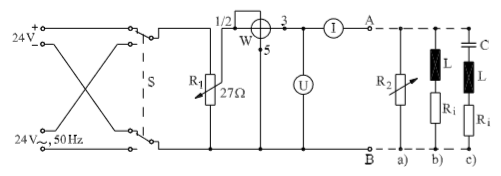
\includegraphics[width=0.9\textwidth]{res/Schaltskizze.png}
	\caption{Schaltskizze, die die im zweiten Teil des Protokolls behandelten Schaltungen beschreibt. }
	\label{fig:Leistungsaufnahme}
\end{figure}

\subsection{Methoden}\label{kap:MethodenS}
%erser Teil
Um die im Zweiten Teil genannten Größen zu berechnen wurde die Spannung $U$, der Strom $I$ und die Leistung $P$ gemessen. 
Die Spannung und der Strom wurden sowohl bei Wechselstrom als auch bei Gleichstrom bestimmt, während die Leistung nur bei Wechselstrom gemessen wurde. Zu beachten ist, dass es sich bei allen im weiteren genannten Werte für $U$,$I$ , die bei Wechselstrom gemessen wurden, um Effektivwerte handelt und $P$ nur gemittelt angegeben werden kann.
Im letzten Teil werden die Werte für die Induktivität und den Innenwiderstand aus dem zweiten Teil übernommen und zusätzlich wurde die Spannung, der Strom und die Leistung bei Wechselstrom aufgenommen.
Die Messungen wurden mit einem Multimeter, einem Ampermeter und einem Wattmeter durchgeführt.
All diese Messgeräte wahren mit einem Analogen Skala versehen. Aus diesem Grund sind alle Unsicherheiten der Messwerte, durch eine Dreiecksverteilung abzuschätzen. 
%Hier wird noch gesagt was für Unsicherheiten wird genau für die Skalen annehmen.
